\documentclass{article}
\usepackage{graphicx} % Required for inserting images
\usepackage[italian]{babel}
\usepackage[hidelinks]{hyperref}
\usepackage{float}
\usepackage{caption}
\usepackage{changepage}
\usepackage{multicol}

\title{Sistemi operativi I}
\author{Leonardo Ganzaroli}
\date{}

\begin{document}

\maketitle

\addcontentsline{toc}{section}{\protect\numberline{}Introduzione}

\tableofcontents

\hypersetup{allcolors=black}

\newpage

\section*{Introduzione}

Questi appunti sono derivanti principalmente dalle slide del corso di \textit{Sistemi operativi I} che ho svolto durante la laurea Triennale di informatica all'università "La Sapienza".\newline

\noindent \textbf{N.B. Questo corso è il naturale proseguimento di \textit{Architettura degli elaboratori}, quindi molte cose saranno date per scontate}.

\newpage

\section{Processi}

\textbf{Definizione} La traccia di un processo è la sua sequenza di istruzioni che vengono eseguite.\newline

\noindent\textbf{Definizione} Il Process Image di un processo è l'insieme di:
\begin{itemize}
    \item \textbf{PCB}
    \item \textbf{Programma sorgente}
    \item \textbf{Dati}
    \item \textbf{Stack delle chiamate}\newline
\end{itemize}

\noindent Per gestire opportunamente i processi il SO mantiene tutti i processi attivi in una tabella, per distinguerli viene assegnato un codice identificativo (PID) ad ognuno.\newline

\noindent\textbf{Definizione} Il dispatcher è un programma che sospende un processo per farne eseguire un altro, usa una o più code per alternare i processi:\newline

\begin{figure}[ht]
    \centering
    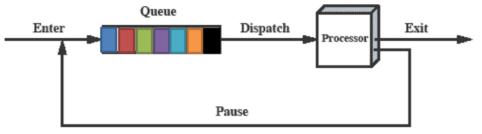
\includegraphics[width=0.7\linewidth]{disp.png}
    \label{fig:disp}
\end{figure}

\noindent Questo presuppone che ogni processo si trovi in un certo stato in ogni istante, scegliendo quali e in che modo si passi da uno stato all'altro porta a diversi modelli, un possibile modello a 5 stati è:\newline

\begin{figure}[ht]
    \centering
    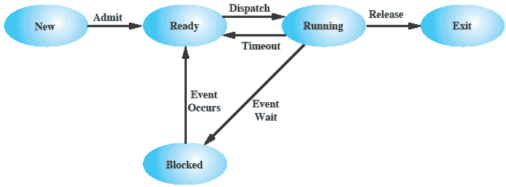
\includegraphics[width=0.8\linewidth]{stat.png}
    \label{fig:stat}
\end{figure}

\newpage

\noindent Per mantenere queste informazioni aggiuntive si estende il PCB in modo che contenga anche:
\begin{itemize}
    \item Identificatori
        \begin{itemize}
            \item \textbf{PID}
            \item \textbf{PPID}
            \item \textbf{Utente proprietario}
        \end{itemize}

    \item Informazioni sullo stato del processore
        \begin{itemize}
            \item \textbf{PSW}
            \item \textbf{Contenuto registri}
        \end{itemize}

    \item Informazioni per il controllo del processo

    \item Supporto per strutture dati

    \item Risorse usate

    \item Permessi speciali

    \item Metodi di comunicazione con altri processi\newline
        
\end{itemize}

\noindent Ogni processore ammette almeno 2 modi di esecuzione per i processi:
\begin{enumerate}
    \item \textbf{Utente}

        Usato per i programmi avviati dall'utente, non permette di svolgere alcune operazioni.
    
    \item \textbf{Sistema}

        Usato dal Kernel, permette di avere pieno controllo ed accedere ad ogni locazione di memoria.
    
\end{enumerate}

\noindent I processi utente possono essere portati in modalità sistema temporaneamente, questo accade quando c'è bisogno di gestire un'interruzione.\newline

\noindent Il SO stesso è trattato come ogni altro programma, l'unica differenza sta nel fatto che possiede dei privilegi più alti. Molto spesso lascia volontariamente il posto ad altri processi per poi riprenderselo tramite interrupt. In particolare i suoi processi vengono eseguiti a livello utente.\newline

\noindent Il Kernel invece viene eseguito al di fuori dei processi ed ha la sua zona di memoria dedicata.\newline

\newpage

\noindent I Thread condividono tutte le risorse del processo padre tranne la stack delle chiamate, possono essere di 3 tipi ed ognuno ha i suoi vantaggi e svantaggi:

\begin{figure}[ht]
    \centering
    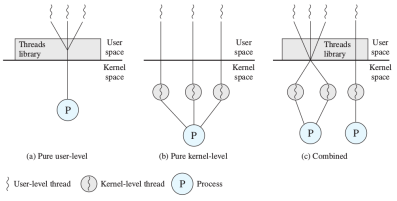
\includegraphics[width=.9\linewidth]{thread.png}
    \label{fig:thread}
\end{figure}

\subsection{Scheduling}

Lo scopo dello scheduling è quello di assegnare i processi da eseguire ad ogni processore, deve farlo nel modo più efficiente possibile ma allo stesso tempo equo per tutti i processi.\newline

\noindent Ne esistono 4 tipi diversi:
\begin{enumerate}

    \item \textbf{I/O}

    Decide l'assegnazione dei dispositivi I/O.

    \item \textbf{A lungo termine}

        Decide quali processi vengono aggiunti a quelli da eseguire.
    
    \item \textbf{A medio termine}

        Decide l'aggiunta di processi nella RAM.
    
    \item \textbf{A breve termine} (dispatcher)

        Decide quale processo tra quelli pronti viene eseguito.\newline
    
\end{enumerate}

\newpage

\noindent L'ultimo è quello eseguito più frequentemente essendo chiamato in risposta agli eventi, i modi per valutare le diverse politiche utilizzabili in questo caso si basano su diversi criteri:
\begin{itemize}
    \item Utente

        \begin{itemize}
            \item Prestazionali

                \begin{itemize}
                    \item \textbf{Tempo di ritorno}

                        Tempo passato tra la creazione ed il completamento di un processo.
                    
                    \item \textbf{Tempo di risposta}

                        Tempo passato tra la sottomissione di una richiesta e l’inizio della risposta.
                        
                    \item \textbf{Deadline}

                        Numero di deadline rispettate.
                    
                \end{itemize}
            
            \item Non prestazionali

                \begin{itemize}
                    \item \textbf{Predicibilità}

                        Variabilità nei tempi di risposta/ritorno.
                    
                \end{itemize}
            
        \end{itemize}
    
    \item Sistema

        \begin{itemize}
            \item Prestazionali

                \begin{itemize}
                    \item \textbf{Throughput}

                        Numero di processi completati per unità di tempo.
                    
                    \item \textbf{Uso del processore}

                        Tempo di utilizzo del processore.

                    
                \end{itemize}
            
            \item Non prestazionali

                \begin{itemize}
                    \item \textbf{Equità}

                        Equità nella gestione dei processi.
                    
                    \item \textbf{Gestione delle priorità}

                        Rispetto delle diverse priorità dei processi.
                            
                    \item \textbf{Bilanciamento delle risorse}

                        Uso delle risorse.\newline
                    
                \end{itemize}
            
        \end{itemize}
    
\end{itemize}

\newpage

\subsubsection{Politiche}

\textbf{Definizione} La funzione di selezione si occupa di scegliere il processo da mandare in esecuzione.\newline

\noindent\textbf{Definizione} La modalità di decisione specifica in quali istanti di tempo viene invocata la precedente, può essere:
\begin{itemize}
    \item \textbf{Preemptive}

        Si può interrompere il processo in qualsiasi momento.
    
    \item \textbf{Non preemptive}

        Si può interrompere solo alla fine dell'esecuzione o in presenza di richieste I/O.\newline
        
\end{itemize}

\noindent Principali politiche di Scheduling:
\begin{itemize}
    \item \textbf{FCFS}
        \begin{itemize}
            \item Alla fine dell'esecuzione si prende il primo processo della coda
            \item Non preemptive
            \item Processi lunghi favoriti
            \item Processi CPU-Bound favoriti
        \end{itemize}

    \item \textbf{Round robin}
            \begin{itemize}
            \item Usa un clock
            \item Ogni processo ha uno slot temporale
            \item Alla fine del suo tempo il processo viene rimesso nella coda
            \item Preemptive
        \end{itemize}

    \item \textbf{Round robin virtuale}

            Come il precedente ma presenta una coda aggiuntiva ad alta priorità, vengono messi in questa coda i processi dopo il completamento di una richiesta I/O con il loro tempo di slot residuo.

    \item \textbf{SPN}
            \begin{itemize}
            \item Si sceglie il processo con tempo stimato di esecuzione minore
            \item Non preemptive
            \item Processi corti favoriti
        \end{itemize}

    \item \textbf{SRT}

        Come il precedente ma preemptive rispetto all'arrivo di un nuovo processo.\newline
        
\end{itemize}

\noindent Nel caso di architetture multiprocessore bisogna gestire anche l'assegnazione dei processi:
\begin{itemize}
    \item \textbf{Statica}

        Gliene viene assegnato uno alla sua creazione.

    \item \textbf{Dinamica}

        La sua esecuzione può variare durante la sua vita.\newline
    
\end{itemize}

\section{Concorrenza}

\textbf{Definizione} Un'operazione atomica è una sequenza indivisibile di comandi.\newline

\noindent\textbf{Definizione} Una sezione critica è una parte di codice che presenta un accesso esclusivo ad una risorsa condivisa.\newline

\noindent\textbf{Definizione} La mutua esclusione è un requisito che impone che un solo processo alla volta sia in una sezione critica.\newline

\noindent\textbf{Definizione} Una race condition è la violazione della mutua esclusione.\newline

\noindent\textbf{Definizione} Il deadlock si verifica quando due o più processi non possono proseguire con l'esecuzione perché si aspettano l'un l'altro.\newline

\noindent\textbf{Definizione} Il livelock si verifica quando due o più processi cambiano continuamente il loro stato (senza fare niente di utile) in risposta agli altri.\newline

\noindent\textbf{Definizione} La starvation si verifica quando un processo \textit{Ready} non viene mai scelto dallo scheduler.\newline

\begin{table}[H]
    \begin{adjustwidth}{-1.5cm}{}
    \begin{tabular}{|c|c|l|}
        \hline
        \textbf{Comunicazione} & \textbf{Relazione} & \multicolumn{1}{|c|}{\textbf{Problemi}}\\
         \hline
        Nessuna & Competizione & Mutua esclusione, deadlock, starvation\\
         \hline
        Memoria condivisa & Cooperazione & Mutua esclusione, deadlock, starvation, coerenza dati\\
         \hline
        Comunicazione primitiva & Cooperazione & Deadlock, starvation\\
         \hline
    \end{tabular}
    \end{adjustwidth}
    \caption{Interazione tra processi}
    \label{tab:conc}
\end{table}

\newpage

\subsection{Mutua esclusione}

Per garantire la mutua esclusione ci sono diversi metodi:
\begin{itemize}
    \item \textbf{Disabilitazione interruzioni} (Solo monoprocessore)

        Se un processo può decidere di non essere interrotto allora nessuno lo può interrompere nella sezione critica. (Possibile peggioramento prestazioni)

    \item \textbf{Istruzioni speciali}

        Si usano delle istruzioni speciali (atomiche) ed una variabile per permettere ad un solo processo alla volta di entrare nella sezione critica.

    \item \textbf{Semafori}

        Una struttura contenente una coda di processi ed un contatore, ha 3 operazioni atomiche associate:
        \begin{enumerate}
            \item \textbf{Initialize}
            \item \textbf{P}
            \item\textbf{V}
        \end{enumerate}

        Quando un processo richiede l'accesso alla risorsa:
        \begin{enumerate}
            \item Chiama P
            \item Se la risorsa è totalmente occupata viene bloccato e messo in coda
            \item Quando un altro processo finisce chiama V
            \item Se la coda non è vuota sveglia un processo e rimuovilo da essa
        \end{enumerate}

        \vspace{10pt}

        Se il contatore assume solo i valori $0,1$ il semaforo viene detto binario.

        \vspace{10pt}

        In base al modo di prelevare i processi dalla coda si identificano 2 tipi:
        \begin{enumerate}
            \item Sem. forte (FIFO)
            \item Sem. debole (Non specificato)
        \end{enumerate}

    \item \textbf{Alg. Dekker} (2 processi)

        Usa 2 flag (una per processo) e una variabile $turno$, $flag_i=true$ indica che il processo $i$ potrebbe essere nella sua fase critica. 

        \vspace{6pt}
        
        Prima della sezione critica un processo controlla la flag dell'altro e se è $true$ aspetta, se il valore di $turno$ è il numero dell'altro processo imposta la propria flag $false$. 

        \vspace{6pt}
        
        Dopo la sezione critica un processo imposta la sua flag $false$ e $turno$ al numero dell'altro processo.

    \item \textbf{Alg. Peterson} (2 processi)

        Versione semplificata del precedente, generalizzazione più semplice.
    
\end{itemize}

\subsection{Interazione}

I processi possono comunicare tra di loro (e potenzialmente sincronizzarsi) tramite l'invio di messaggi, lo scambio avviene tramite le operazioni atomiche:
\begin{itemize}
    \item \textbf{Send}
    \item \textbf{Receive}
\end{itemize}

\noindent Lo scambio di un messaggio può essere:
\begin{itemize}
    \item \textbf{Bloccante} 

        I 2 processi coinvolti si bloccano fino alla ricezione del messaggio.

    \item \textbf{Non bloccante}

        La ricezione può essere bloccante o meno, l'invio non lo è.\newline 
    
\end{itemize}

\noindent Per indirizzare il messaggio ci sono 2 metodi:
\begin{enumerate}
    \item \textbf{Diretto}

        Si specifica un identificatore, ogni processo ha una sua coda.

    \item \textbf{Indiretto}

        I messaggi vengono inviati ad una mailbox condivisa, va creata esplicitamente.\newline
    
\end{enumerate}

\begin{figure}[ht]
    \centering
    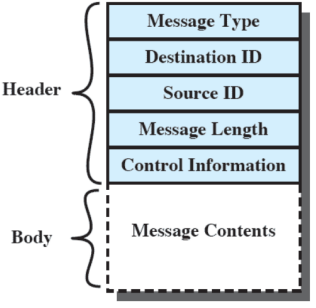
\includegraphics[width=0.4\linewidth]{msg.png}
    \caption{Formato tipico messaggio}
    \label{fig:msg}
\end{figure}

\noindent In generale tutti i metodi visti sono intercambiabili tra loro per quanto riguarda la condivisione di risorse. 

\subsection{Deadlock}

Le risorse si possono classificare in:
\begin{itemize}
    \item \textbf{Riusabili}
        \begin{itemize}
            \item Usabili da un solo processo alla volta
            \item Non vengono "consumate"
        \end{itemize}

    \item \textbf{Non riusabili}
        \begin{itemize}
            \item Vengono create e distrutte
        \end{itemize}
\end{itemize}

\vspace{3pt}

\noindent Il deadlock nei 2 casi può avvenire rispettivamente se:
\begin{itemize}
    \item Un processo che sta usando una risorsa ne richiede un'altra
    \item Viene richiesta una risorsa non ancora creata\newline
\end{itemize}

\noindent Lo stato delle risorse e dei processi può essere rappresentato tramite un grafo in cui:
\begin{itemize}
    \item Un cerchio rappresenta un processo
    \item Un rettangolo rappresenta una risorsa
    \item Un pallino nel rettangolo rappresenta un'istanza della risorsa
    \item Un arco Processo $\rightarrow$ Risorsa è una richiesta
    \item Un arco Risorsa $\rightarrow$ Processo è un'assegnazione\newline
\end{itemize}

\begin{figure}[ht]
    \centering
    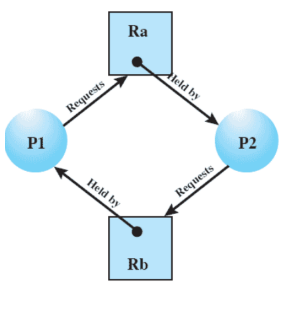
\includegraphics[width=0.4\linewidth]{dead.png}
    \caption{Esempio di deadlock}
    \label{fig:deadlock}
\end{figure}

\noindent Oltre a cercare di prevenirlo si può provare ad evitarlo (ad esempio con l'algoritmo del banchiere), nel caso si verifichi comunque si possono terminare i processi coinvolti, usare punti di ripristino oppure prendere forzatamente le loro risorse.

\section{I/O}

Data l'esistenza di svariati tipi di dispositivi I/O che possono presentare caratteristiche anche estremamente diverse tra loro risulta complicato catalogarli, a grandi linee però si possono dividere in:
\begin{itemize}
    \item Comunicazione diretta con l'utente
    \item Comunicazione con dispositivi elettronici
    \item Comunicazione con dispositivi remoti\newline
\end{itemize}

\noindent Un'altra possibilità è l'uso di una gerarchia che presenta delle similitudini con i protocolli usati nelle reti:
\begin{enumerate}
    \item \textbf{Dispositivi locali}
    \item \textbf{Dispositivi di comunicazione}
    \item \textbf{File System}\newline
\end{enumerate}

\noindent Per evitare situazioni di deadlock dovute a richieste I/O delle pagine in memoria si può usare il \textit{buffering}, ossia avere dei buffer in memoria (spazio di sistema). Questo potenzialmente permette di avere l'input già pronto prima della richiesta e di posticipare l'output.\newline

\begin{figure}[ht]
    \centering
    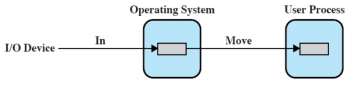
\includegraphics[width=0.6\linewidth]{b1.png}
    \caption*{Singolo}
    \vspace{10pt}
    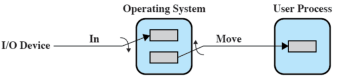
\includegraphics[width=0.6\linewidth]{b2.png}
    \caption*{Doppio}
    \vspace{10pt}
    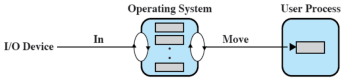
\includegraphics[width=0.6\linewidth]{b3.png}
    \caption*{Circolare}
    
    \label{fig:buf}
\end{figure}

\newpage

\subsection{Gestione del disco}

Dato il suo funzionamento il disco rigido presenta dei tempi di ricerca/scrittura che possono risultare lunghi, usando opportune politiche di gestione delle richieste si può ottimizzare il processo:
\begin{itemize}
    \item \textbf{RSS}

        Scheduling random.
        
    \item \textbf{FIFO}    
    \item \textbf{LIFO}
    \item \textbf{Priorità}

    \item \textbf{SSTF}

        Si sceglie la richiesta che provoca il minore spostamento della testina.

    \item \textbf{SCAN}

        Si scelgono le richieste in modo che la testina vada sempre in un verso, quando arriva al bordo procede nel verso opposto.

    \item \textbf{C-SCAN}

        Come il precedente ma nel ritorno non si svolgono richieste.

    \item \textbf{FSCAN}

        Ogni nuova richiesta deve aspettare che tutte le precedenti vengano eseguite, si usano 2 code per fare ciò.

    \item \textbf{N-step SCAN}

        Generalizzazione del precedente con più di 2 code.\newline
        
\end{itemize}

\noindent Un ulteriore meccanismo prevede di usare un buffer in memoria per mantenere alcune settori del disco, le politiche di rimpiazzo sono le stesse della Cache.\newline

\subsubsection{RAID}

\textbf{Definizione} Uno strip è un insieme di settori.\newline

\noindent\textbf{Definizione} Uno stripe è un insieme di strip.\newline

\noindent\textbf{Definizione} Un blocco è uno strip potenzialmente grande.\newline

\noindent\textbf{Definizione} Il \textit{Redundant Array of Independent Disks} è un metodo che permette di usare un insieme di dischi come se fossero uno.

\newpage

\noindent Le configurazioni principali sono:
\begin{itemize}
    \item \textbf{RAID0}

        I dati vengono distribuiti per avere un accesso più efficiente.

        \begin{figure}[ht]
            \centering
            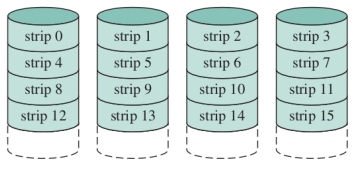
\includegraphics[width=0.5\linewidth]{r1.png}
            \label{fig:raid0}
        \end{figure}

    \item \textbf{RAID1}

        Come il precedente ma i dati vengono duplicati.

        \begin{figure}[ht]
            \centering
            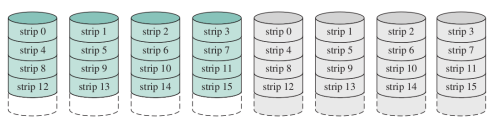
\includegraphics[width=0.9\linewidth]{r2.png}
            \label{fig:raid1}
        \end{figure}

    \item \textbf{RAID2}

        Ridondanza tramite codice di Hamming.

        \begin{figure}[ht]
            \centering
            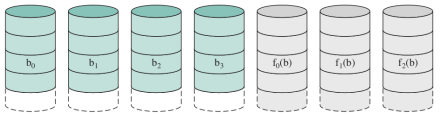
\includegraphics[width=0.8\linewidth]{r3.png}
            \label{fig:raid2}
        \end{figure}

    \item \textbf{RAID3}

        Ridondanza (byte) tramite un disco che contiene le parità.

        \begin{figure}[H]
            \centering
            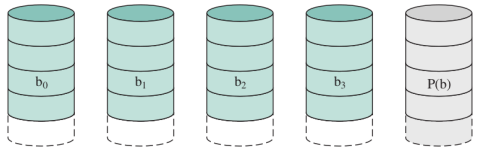
\includegraphics[width=0.7\linewidth]{r4.png}
            \label{fig:raid3}
        \end{figure}

    \newpage

    \item \textbf{RAID4}

        Generalizzazione del precedente.

        \begin{figure}[ht]
            \centering
            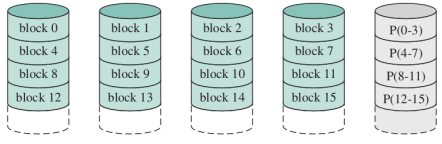
\includegraphics[width=0.8\linewidth]{r5.png}
            \label{fig:raid4}
        \end{figure}

    \item \textbf{RAID5}

        Come il precedente ma senza un disco dedicato, le parità sono distribuite.

        \begin{figure}[ht]
            \centering
            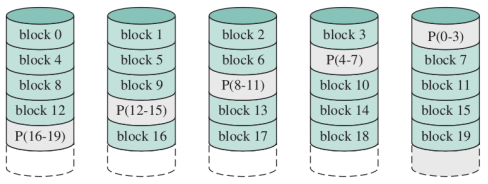
\includegraphics[width=0.8\linewidth]{r6.png}
            \label{fig:raid5}
        \end{figure}

    \item \textbf{RAID6}

        Come il precedente ma le parità sono duplicate.\newline

        \begin{figure}[ht]
            \centering
            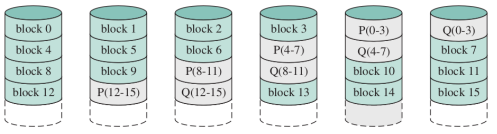
\includegraphics[width=0.9\linewidth]{r7.png}
            \label{fig:raid6}
        \end{figure}
    
\end{itemize}

\newpage

\section{File system}

\textbf{Definizione} Campo = uno o più dati base.\newline

\noindent\textbf{Definizione} Metadato = dato che descrive una proprietà di un altro dato.\newline

\noindent\textbf{Definizione} Record = insieme di campi correlati.\newline

\noindent\textbf{Definizione} File = insieme di record correlati.\newline

\noindent\textbf{Definizione} Database = collezione di dati correlati.\newline

\noindent\textbf{Definizione} Volume = disco logico = insieme di settori.\newline

\noindent\textbf{Definizione} Il \textit{File Management System} si occupa di fornire servizi all'utente ed alle applicazioni che permettono di interagire con i file.\newline

\noindent\textbf{Definizione} Una directory è un file speciale che contiene altri file, in particolare deve contenere tutte le loro informazioni e fornire un mapping tra un nome ed il file corrispondente.\newline

\noindent L'assegnazione di memoria secondaria ad un file comporta gli stessi problemi visti per quella primaria, similmente si può usare un'allocazione statica/dinamica con blocchi fissi/variabili.\newline

\noindent Per allocare i blocchi effettivi ci sono diversi metodi:
\begin{itemize}
    \item \textbf{Contigua}

        I blocchi necessari sono tutti in sequenza, possibile frammentazione esterna.

        \begin{figure}[ht]
            \begin{minipage}[t]{0.5\textwidth}
                \centering
                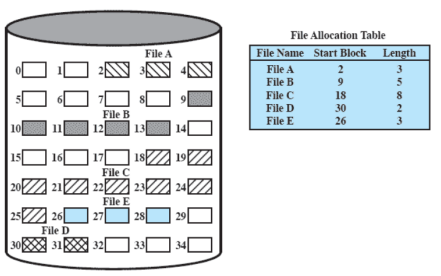
\includegraphics[width=\linewidth]{cont.png}
            \end{minipage}
            \vrule width 1pt\hspace{0.5em}
            \hfill
            \begin{minipage}[t]{0.5\textwidth}
                \centering
                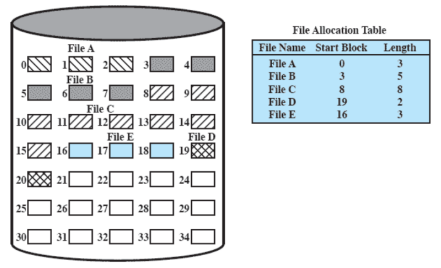
\includegraphics[width=\linewidth]{cont2.png}
                \caption*{Dopo compattazione}
            \end{minipage}
        \end{figure}

    \newpage

    \item \textbf{Concatenata}

        Ogni blocco contiene un puntatore al prossimo.

        \begin{figure}[ht]
            \begin{minipage}[t]{0.5\textwidth}
                \centering
                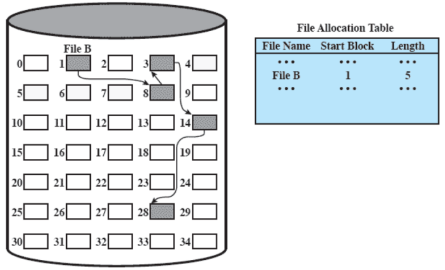
\includegraphics[width=\linewidth]{concat.png}
            \end{minipage}
            \vrule width 1pt\hspace{0.5em}
            \hfill
            \begin{minipage}[t]{0.5\textwidth}
                \centering
                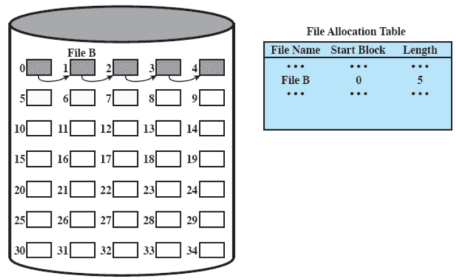
\includegraphics[width=\linewidth]{concat2.png}
                \caption*{Dopo consolidamento}
            \end{minipage}
        \end{figure}

    \item \textbf{Indicizzata}

        Viene usato un blocco indice che contiene gli indirizzi degli altri blocchi.\newline

        \begin{figure}[ht]
            \begin{minipage}[t]{0.5\textwidth}
                \centering
                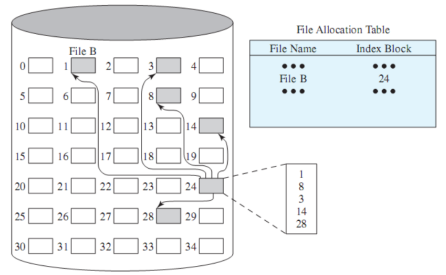
\includegraphics[width=\linewidth]{ind.png}
                \caption*{Porzioni fisse}
            \end{minipage}
            \vrule width 1pt\hspace{0.5em}
            \hfill
            \begin{minipage}[t]{0.5\textwidth}
                \centering
                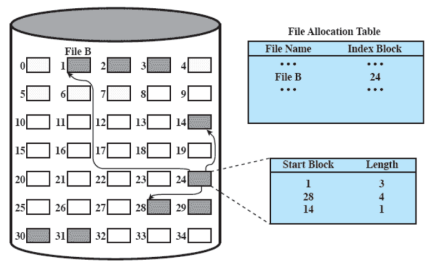
\includegraphics[width=\linewidth]{ind2.png}
                \caption*{Porzioni variabili}
            \end{minipage}
        \end{figure}
    
\end{itemize}

\noindent Per far funzionare questi metodi bisogna mantenere una lista dei file ed una per i blocchi liberi, quest'ultima può essere implementata tramite:
\begin{itemize}
    \item \textbf{Lista dei blocchi liberi}
    \item \textbf{Tabella di bit}

        Vettore con un bit associato ad ogni blocco, 0 se libero.
    
    \item \textbf{Porzioni libere concatenate}

        Si concatenano i blocchi liberi con i puntatori, bisogna specificare la dimensione del blocco puntato.
    
    \item \textbf{Indicizzazione}

        Tutto lo spazio libero viene visto come un file.\newline
    
\end{itemize}

\noindent\textbf{Definizione} Il Journaling è una tecnica per preserva l'integrità dei dati in caso di problemi, prima di effettuare un'operazione viene scritta la stessa in una zona designata in memoria (log). In questo modo se per esempio non viene portata a termine per uno spegnimento improvviso il SO la porterà a termine alla successiva accensione leggendo il log.

\end{document}
